\documentclass[a4paper, 12pt]{article}

\usepackage[pdftex]{hyperref}
\usepackage{graphicx}
\usepackage{float}

\title{Arquitetura de Software}
\author{João Vitor Espig}

\begin{document}
    \maketitle
    \section{Conteúdo}
    seção de conteúdo

    O projeto tem o \textit{front-end} feito utilizando \textit{HTML}, \textit{CSS} e \textit{Javascript} -- as linguagens mais comuns nos dias atuais para o desenvolvimento de páginas \textit{web} -- e o \textit{back-end} feito utilizando \textit{Go}(\textit{Lang}), uma linguagem de programação compilada que prioriza o desenvolvimento de aplicações de alta performance [1] e tem um processo de desenvolvimento rápido por conta de sua simplicidade [2]. Dentro do ambiente de desenvolvimento é utilizado o SQLite3 como banco de dados, por conta de ser simples, leve e de simples configuração e utilização [3].

    O sistema foi divido em módulos e submódulos para uma melhor organização e entendimento por parte dos autores. O módulo principal do projeto é o agendamento, que é o escopo de maior importância para o SISAE. O módulo agendamento foi planejado para ser o mais conciso possível, com o intuito de ser de simples uso e manutenção. A Figura~\ref{fig:umldiagram} apresenta o diagram UML proposto para a abordagem feita no desenvolvimento.

    \begin{figure}[H]
        \begin{center}
            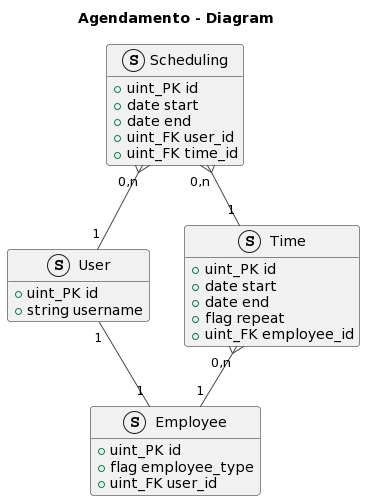
\includegraphics[width=0.5\textwidth]{uml-diagram-img}
        \end{center}
        \caption{Diagrama do agendamento.}
        \label{fig:umldiagram}
    \end{figure}

    \newpage
    \section{Referências}

    \begingroup
    \fontsize{10}{12}\selectfont
        [1] - \url{https://www.w3schools.com/go/go_introduction.php}

        [2] - \url{https://jeffotoni.medium.com/golang-simplificando-a-complexidade-o-inicio-145371d67711}

        [3] - \url{https://rockcontent.com/br/blog/sqlite/#:~:text=O%20SQLite%20%C3%A9%20uma%20base,tr%C3%A1fego%20m%C3%A9dio%20e%20sistemas%20mobile.}
    \endgroup
\end{document}
